%\documentclass[t,10pt]{beamer}
\documentclass[t,handout]{beamer}

\usepackage{graphicx}
\usepackage{epsfig}
\usepackage{psfrag}
\usepackage[english]{babel}
\usepackage{color}
\usepackage{natbib}
\usepackage{booktabs}
\usepackage{listings}

% Font settings:
\usepackage[T1]{fontenc}
\usepackage{mathptmx}
\usepackage[scaled]{helvet}
\usepackage{courier}
\usepackage{microtype}



%Mathematics packages
\usepackage{amsmath}
\usepackage{mathrsfs}
\usepackage{amsfonts}
\usepackage{enumerate}

\graphicspath{{./images/}} % Figures path - used in graphicx

\selectcolormodel{cmyk}

\mode<presentation>

%THEMES - Please refer to these chapters in the beamer documentation.
% Presentation themes : Chapter 15
% Color themes : Chapter 17
% Font themes : Chapter 18
\usetheme{Pittsburgh}
\usecolortheme{orchid}
\usefonttheme{default}

\setbeamertemplate{bibliography item}[text]
\setbeamercovered{transparent=7}

%---------------------------Title frame definition------------------------------------- 

\title{Information Protection in Content-centric Networks}
\author [Chris]{Christopher C. Lamb}
\institute[University of New Mexico]{
\inst {}Department of Electrical and Computer Engineering\\
University of New Mexico}
\date{November 6, 2012}
\titlegraphic{
\begin{figure} 

\includegraphics[width = 7cm]{UNM}
\end{figure}}

% Delete this, if you do not want the table of contents to pop up at
% the beginning of each subsection:
%\AtBeginSubsection[]
%{
%  \begin{frame}<beamer>
%    \frametitle{Outline}
%     \tableofcontents[currentsection,currentsubsection]
%  \end{frame}
%}

\begin{document}

\begin{frame}
\titlepage
\end{frame}

% This command will make the logo appear on all frames excluding the title frame.
\logo {
\includegraphics[width = 2.5cm]{UNM}}

\begin{frame}
\frametitle{Networks in the Bad Old Days}
\begin{figure}[!t]
\centering
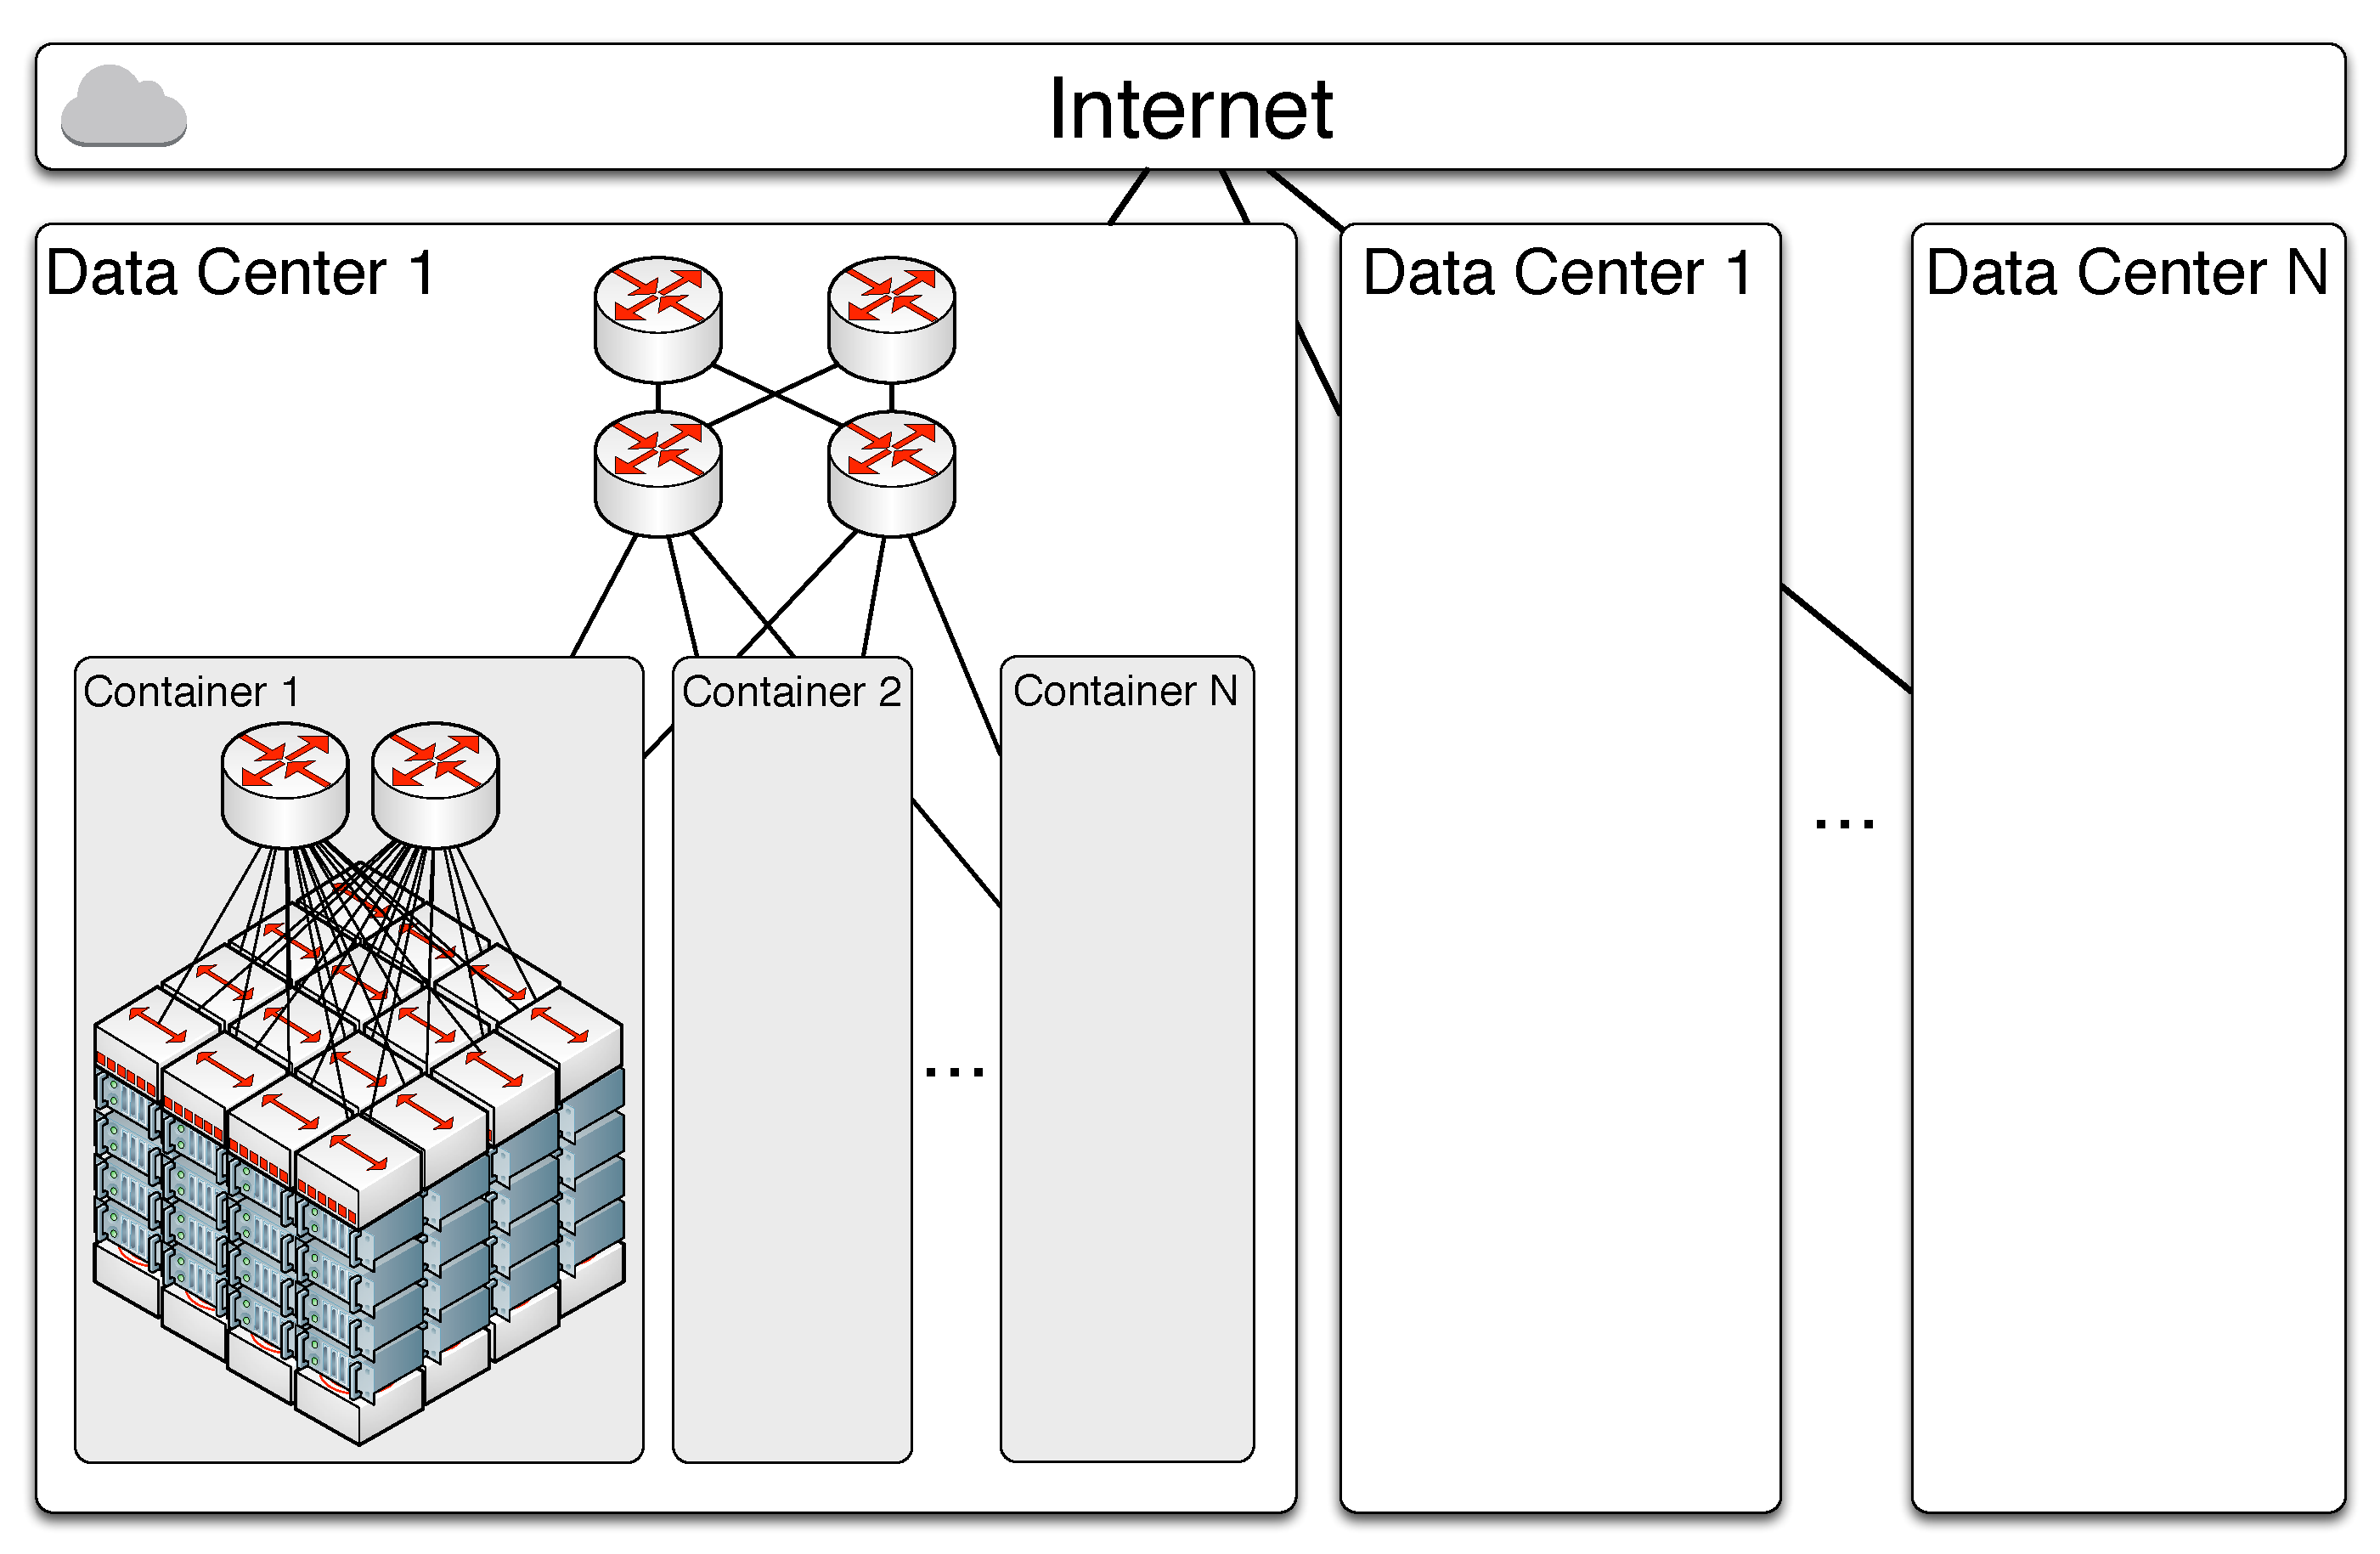
\includegraphics[height=2.75in]{lrg-network}
%\caption{Hierarchical Results from Comcast}
\end{figure}
\end{frame}

\begin{frame}
\frametitle{The Brave New World!}
\begin{figure}[!t]
\centering
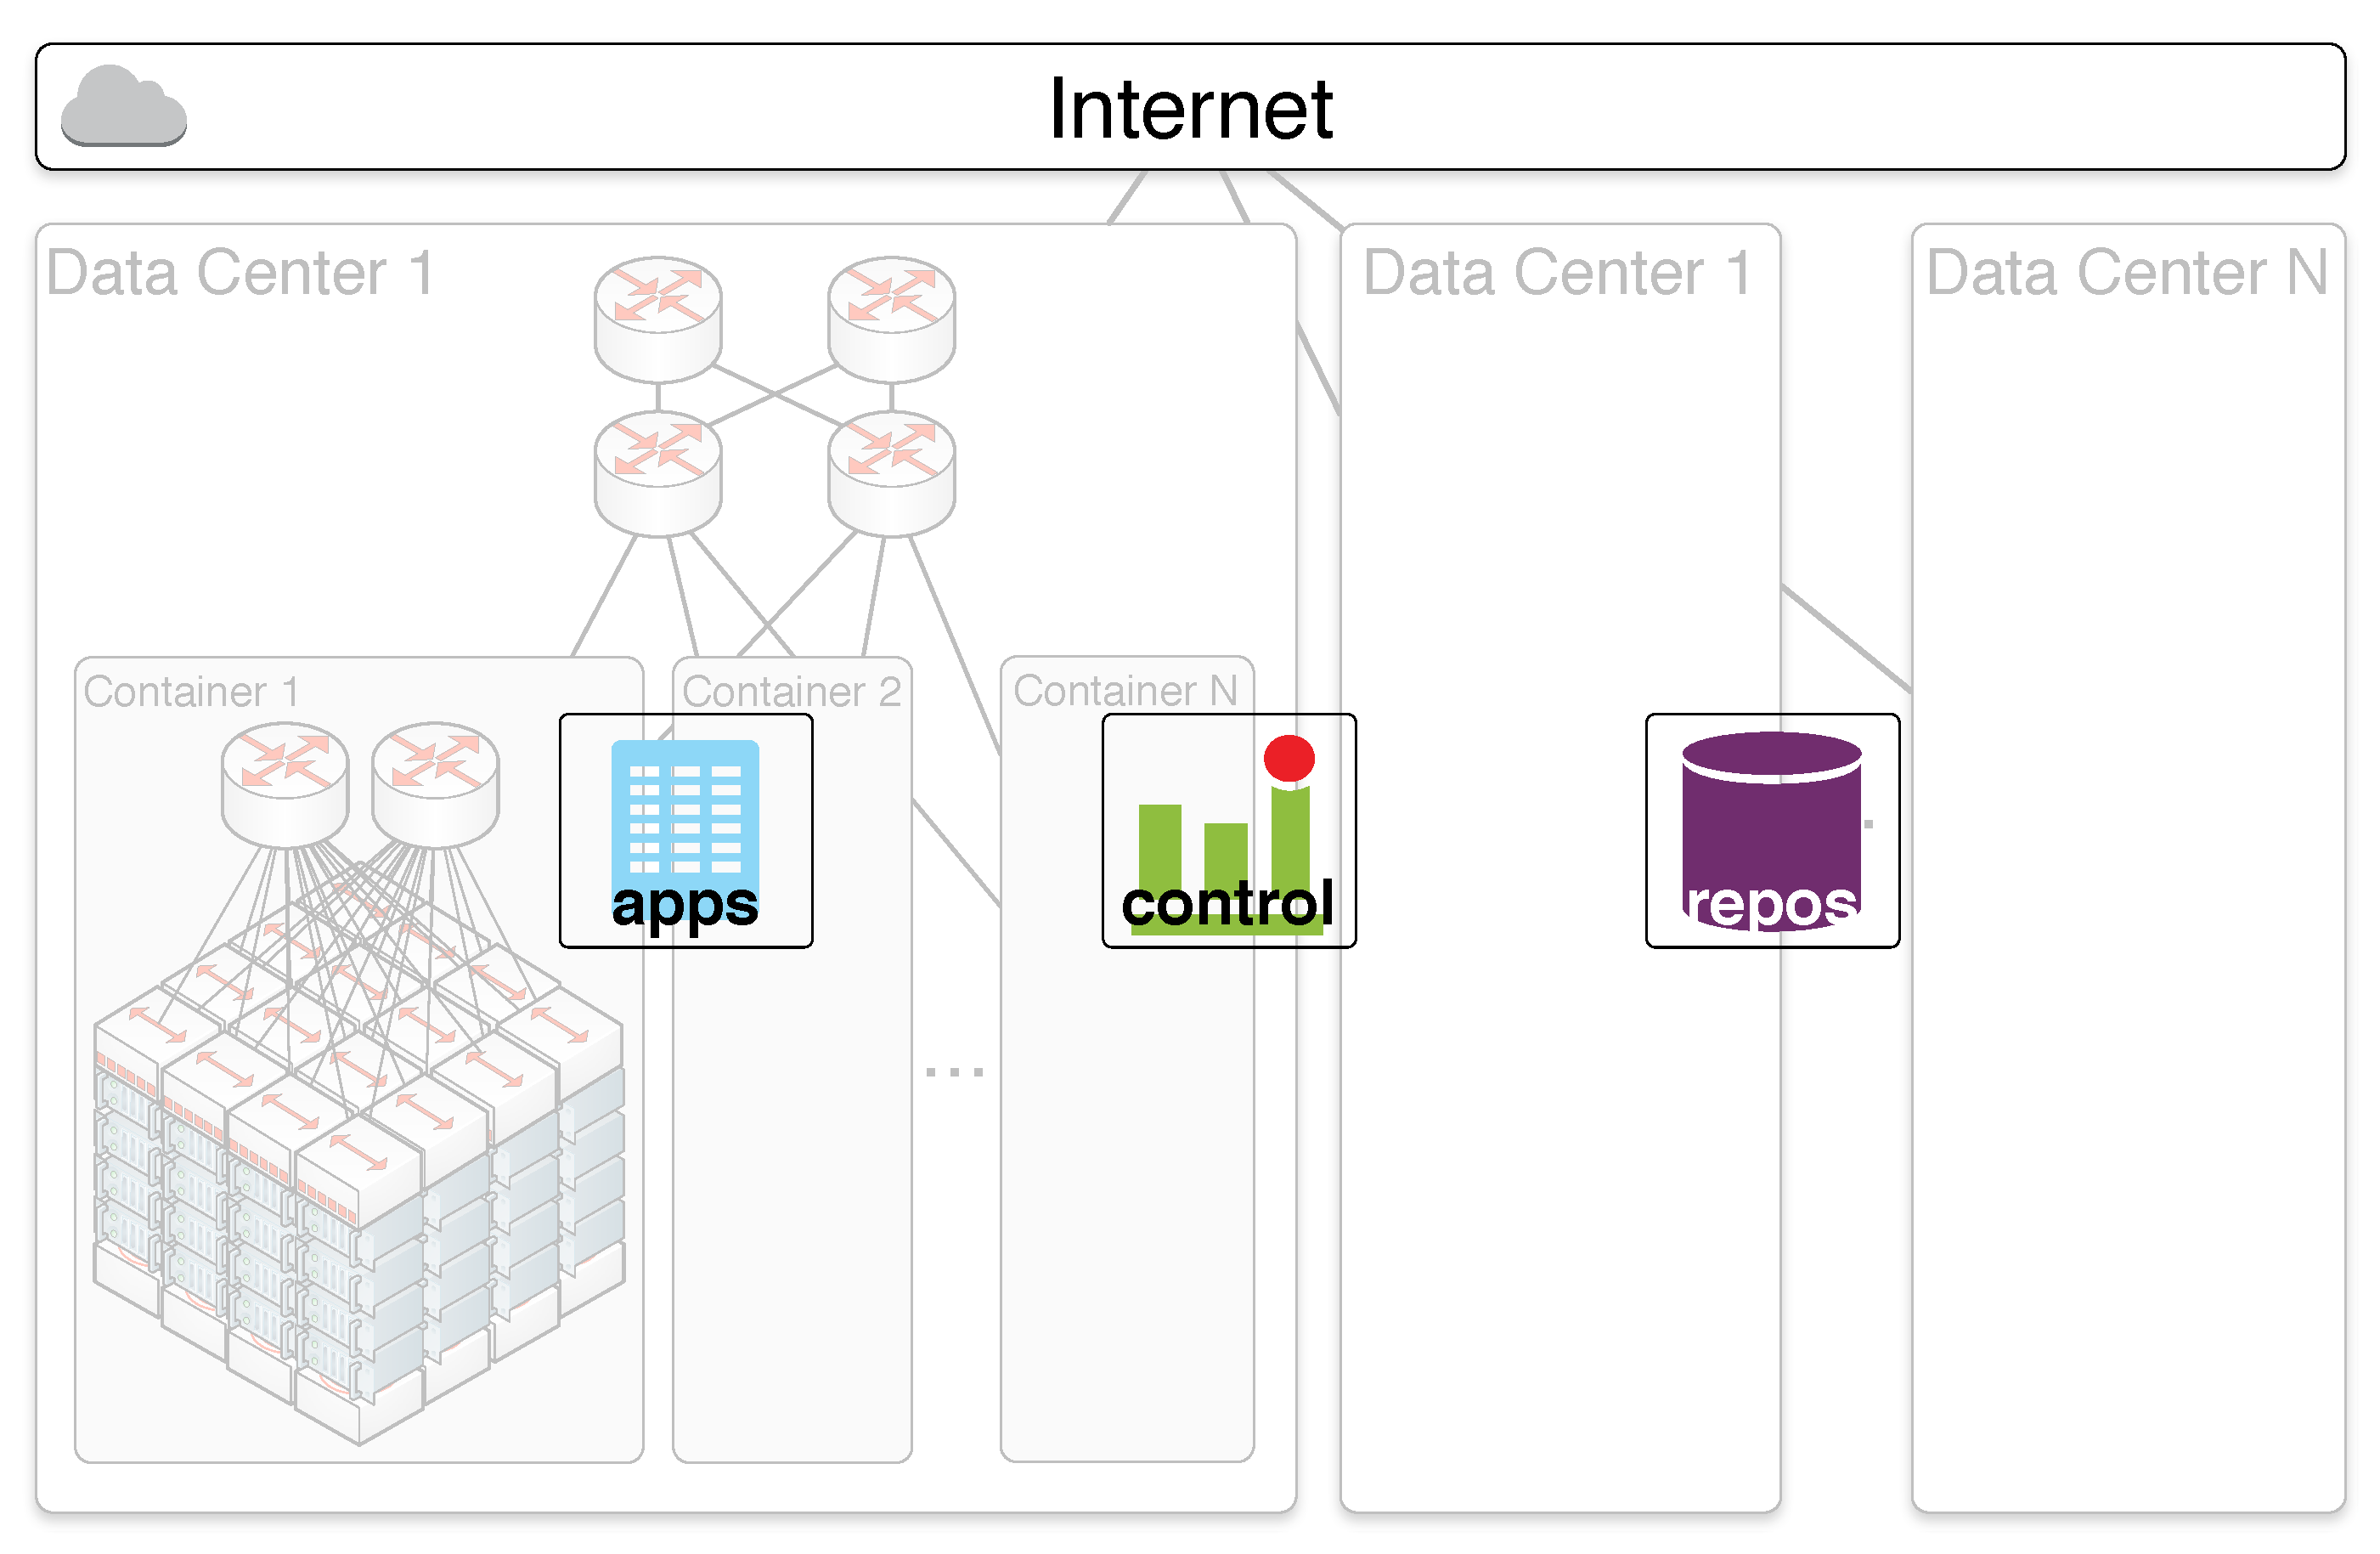
\includegraphics[height=2.75in]{lrg-network-sdn}
%\caption{Hierarchical Results from Comcast}
\end{figure}
\end{frame}

\begin{frame}
\frametitle{Original Goals}
\begin{beamerboxesrounded}[shadow]{Contribution of Work}
The contribution of this work is a quantitative analysis of policy-centric overlay network options, associated taxonomies of use, and prototypical technology proofs-of-concept.
\end{beamerboxesrounded}
\begin{itemize}
\item \textit{Network Control Options} --- {\small This includes various types networks and associated strengths and weaknesses addressing centralized and decentralized models.}
\item \textit{Taxonomies of Use} --- {\small Depending on the specific usage management requirements and context, different overlays have different applicability; this work will provide guidance on suitability; it will eventually lead to how to manage data flow within SDN-capable infrastructure.}
\item \textit{Prototypical Technologies} --- {\small Examples and proofs-of-concept will be required to appropriately analyze various architectural alternatives.}
\end{itemize}
\end{frame}

\begin{frame}
\frametitle{Meeting the Goals}
\begin{beamerboxesrounded}[shadow]{Network Control Options}
{\small I have developed and analysed multiple types of overlay systems, both centralized (hierarchical) and non-centralized (non-hierarchical), with differing topologies and integrated content-centric control.}
\end{beamerboxesrounded}
~\\
\begin{beamerboxesrounded}[shadow]{Taxonomies of Use}
{\small I have established and verified a taxonomy of usage management and applied that within the network providing mechanisms extendible to SDN use.}
\end{beamerboxesrounded}
~\\
\begin{beamerboxesrounded}[shadow]{Prototypical Technologies}
{\small Prototype information-centric networks are running between the Rackspace and Amazon clouds.}
\end{beamerboxesrounded}
\end{frame}

\begin{frame}
\frametitle{Impact and Originality}
\begin{itemize}
\item Information-centric architectures common in future internet designs
\item Significant work with respect to name/object binding, overall topologies, approaches
\item No significant work yet on exploiting new capabilities in information-centricity for enhanced security
\begin{itemize}
\item {\small Absense of strict layering}
\item {\small Lack of packetization preserves contexts} 
\item {\small Evolution of end-to-end arguments}
\end{itemize}
\end{itemize}
\begin{beamerboxesrounded}[shadow]{Additional Contributions}
{\small This work, as well as providing alternatives analysis with respect to security in information-centric architectures and approaches, also demonstrates the first implementation of granular context-sensitive security functionality embedded in an information-centric network.}
\end{beamerboxesrounded}
\end{frame}



\begin{frame}[c]
\begin{center}
\textbf{Questions? Comments?}
\end{center}
\end{frame}

%\input{content-slides/references}

\end{document}

